\documentclass[10pt]{article}  

%%%%%%%% PREÁMBULO %%%%%%%%%%%%
\title{Plantilla para prácticas de UGR}
\usepackage[spanish]{babel} %Indica que escribiermos en español
\usepackage[utf8]{inputenc} %Indica qué codificación se está usando ISO-8859-1(latin1)  o utf8  
\usepackage{amsmath} % Comandos extras para matemáticas (cajas para ecuaciones,
% etc)
\usepackage{amssymb} % Simbolos matematicos (por lo tanto)
\usepackage{graphicx} % Incluir imágenes en LaTeX
\usepackage{color} % Para colorear texto
\usepackage{subfigure} % subfiguras
\usepackage{float} %Podemos usar el especificador [H] en las figuras para que se
% queden donde queramos
\usepackage{capt-of} % Permite usar etiquetas fuera de elementos flotantes
% (etiquetas de figuras)
\usepackage{sidecap} % Para poner el texto de las imágenes al lado
	\sidecaptionvpos{figure}{c} % Para que el texto se alinie al centro vertical
\usepackage{caption} % Para poder quitar numeracion de figuras
\usepackage{commath} % funcionalidades extras para diferenciales, integrales,
% etc (\od, \dif, etc)
\usepackage{cancel} % para cancelar expresiones (\cancelto{0}{x})

\graphicspath{{/Users/jesusgarciamanday/Desktop/Master/CC-II/Practicas/Practica4/p4/Imagenes/}}

\usepackage{anysize} 					% Para personalizar el ancho de  los márgenes
\marginsize{2cm}{2cm}{2cm}{2cm} % Izquierda, derecha, arriba, abajo

\usepackage{appendix}
\renewcommand{\appendixname}{Apéndices}
\renewcommand{\appendixtocname}{Apéndices}
\renewcommand{\appendixpagename}{Apéndices} 

% Para que las referencias sean hipervínculos a las figuras o ecuaciones y
% aparezcan en color
\usepackage[colorlinks=true,plainpages=true,citecolor=blue,linkcolor=blue]{hyperref}
%\usepackage{hyperref} 
% Para agregar encabezado y pie de página
\usepackage{fancyhdr} 
\pagestyle{fancy}
\fancyhf{}
\fancyhead[L]{\footnotesize UGR} %encabezado izquierda
\fancyhead[R]{\footnotesize CCIA}   % dereecha
\fancyfoot[R]{\footnotesize Pr\'actica 4 - Hadoop }  % Pie derecha
\fancyfoot[C]{\thepage}  % centro
\fancyfoot[L]{\footnotesize Master en Ingenier\'ia Inform\'atica }  %izquierda
\renewcommand{\footrulewidth}{0.4pt}


\usepackage{listings} % Para usar código fuente
\definecolor{dkgreen}{rgb}{0,0.6,0} % Definimos colores para usar en el código
\definecolor{gray}{rgb}{0.5,0.5,0.5} 
% configuración para el lenguaje que queramos utilizar
\lstset{language=Matlab,
   keywords={break,case,catch,continue,else,elseif,end,for,function,
      global,if,otherwise,persistent,return,switch,try,while},
   basicstyle=\ttfamily,
   keywordstyle=\color{blue},
   commentstyle=\color{red},
   stringstyle=\color{dkgreen},
   numbers=left,
   numberstyle=\tiny\color{gray},
   stepnumber=1,
   numbersep=10pt,
   backgroundcolor=\color{white},
   tabsize=4,
   showspaces=false,
   showstringspaces=false}

\newcommand{\sen}{\operatorname{\sen}}	% Definimos el comando \sen para el seno
%en español

\title{Práctica 4 - Computación escalable y distribuida con Hadoop}

%%%%%%%% TERMINA PREÁMBULO %%%%%%%%%%%%

\begin{document}

%%%%%%%%%%%%%%%%%%%%%%%%%%%%%%%%%% PORTADA %%%%%%%%%%%%%%%%%%%%%%%%%%%%%%%%%%%%%%%%%%%%
																					%%%
\begin{center}																		%%%
\newcommand{\HRule}{\rule{\linewidth}{0.5mm}}									%%%\left
 																					%%%
\begin{minipage}{0.48\textwidth} \begin{flushleft}
%
\includegraphics[scale = 0.63]{Imagenes/logo_upiita}
\end{flushleft}\end{minipage}
\begin{minipage}{0.48\textwidth} \begin{flushright}
%
\includegraphics[scale = 0.35]{Imagenes/IPN}
\end{flushright}\end{minipage}

													 								%%%
\vspace*{-1.5cm}								%%%
																					%%%	
\textsc{\huge Universidad de\\ \vspace{5px} Granada}\\[1.5cm]	

\textsc{\LARGE Master Profesional en Ingenier\'ia Inform\'atica }\\[1.5cm]													%%%

\begin{minipage}{0.9\textwidth} 
\begin{center}																					%%%
\textsc{\LARGE Pr\'actica 2}
\end{center}
\end{minipage}\\[0.5cm]
%%%
    																				%%%
 			\vspace*{1cm}																		%%%
																					%%%
\HRule \\[0.4cm]																	%%%
{ \huge \bfseries Hadoop}\\[0.4cm]	%%%
 																					%%%
\HRule \\[1.5cm]																	%%%
 																				%%%
																					%%%
\begin{minipage}{0.46\textwidth}													%%%
\begin{flushleft} \large															%%%
\emph{Autor:}\\	
Manuel Jes\'us Garc\'ia Manday (nickter@correo.ugr.es)\\
%%%
			%\vspace*{2cm}	
            													%%%
										 						%%%
\end{flushleft}																		%%%
\end{minipage}		
																%%%
\begin{minipage}{0.52\textwidth}		
\vspace{-0.6cm}											%%%
\begin{flushright} \large															%%%
													%%%
\end{flushright}																	%%%
\end{minipage}	
\vspace*{1cm}
%\begin{flushleft}
 	
%\end{flushleft}
%%%
 		\flushleft{\textbf{\Large Master en Ingenier\'ia Inform\'atica}	}\\																		%%%
\vspace{2cm} 																				
\begin{center}																					
{\large \today}																	%%%
 			\end{center}												  						
\end{center}							 											
																					
\newpage																		
%%%%%%%%%%%%%%%%%%%% TERMINA PORTADA %%%%%%%%%%%%%%%%%%%%%%%%%%%%%%%%

\tableofcontents 

\newpage

\section{Objetivo.}
El objetivo de esta práctica es realizar programas escalables para mejorar la eficiencia en entornos Big Data.\\


\section{Introduccíon.}
Para comenzar a realizar las tareas  que se piden en esta práctica, es necesario en primer lugar realizar una serie de pasos iniciales que se describen a continuación. \\

Realizamos una conexión remota hacía el servidor \textbf{haddop.ugr.es} y una vez dentro creamos una carpeta nueva donde descargaremos el código Java de los programas. Comprobamos tambien que los datos de entrada se encuentran disponibles.\\

 \begin{figure}[H]
	\begin{center}
 		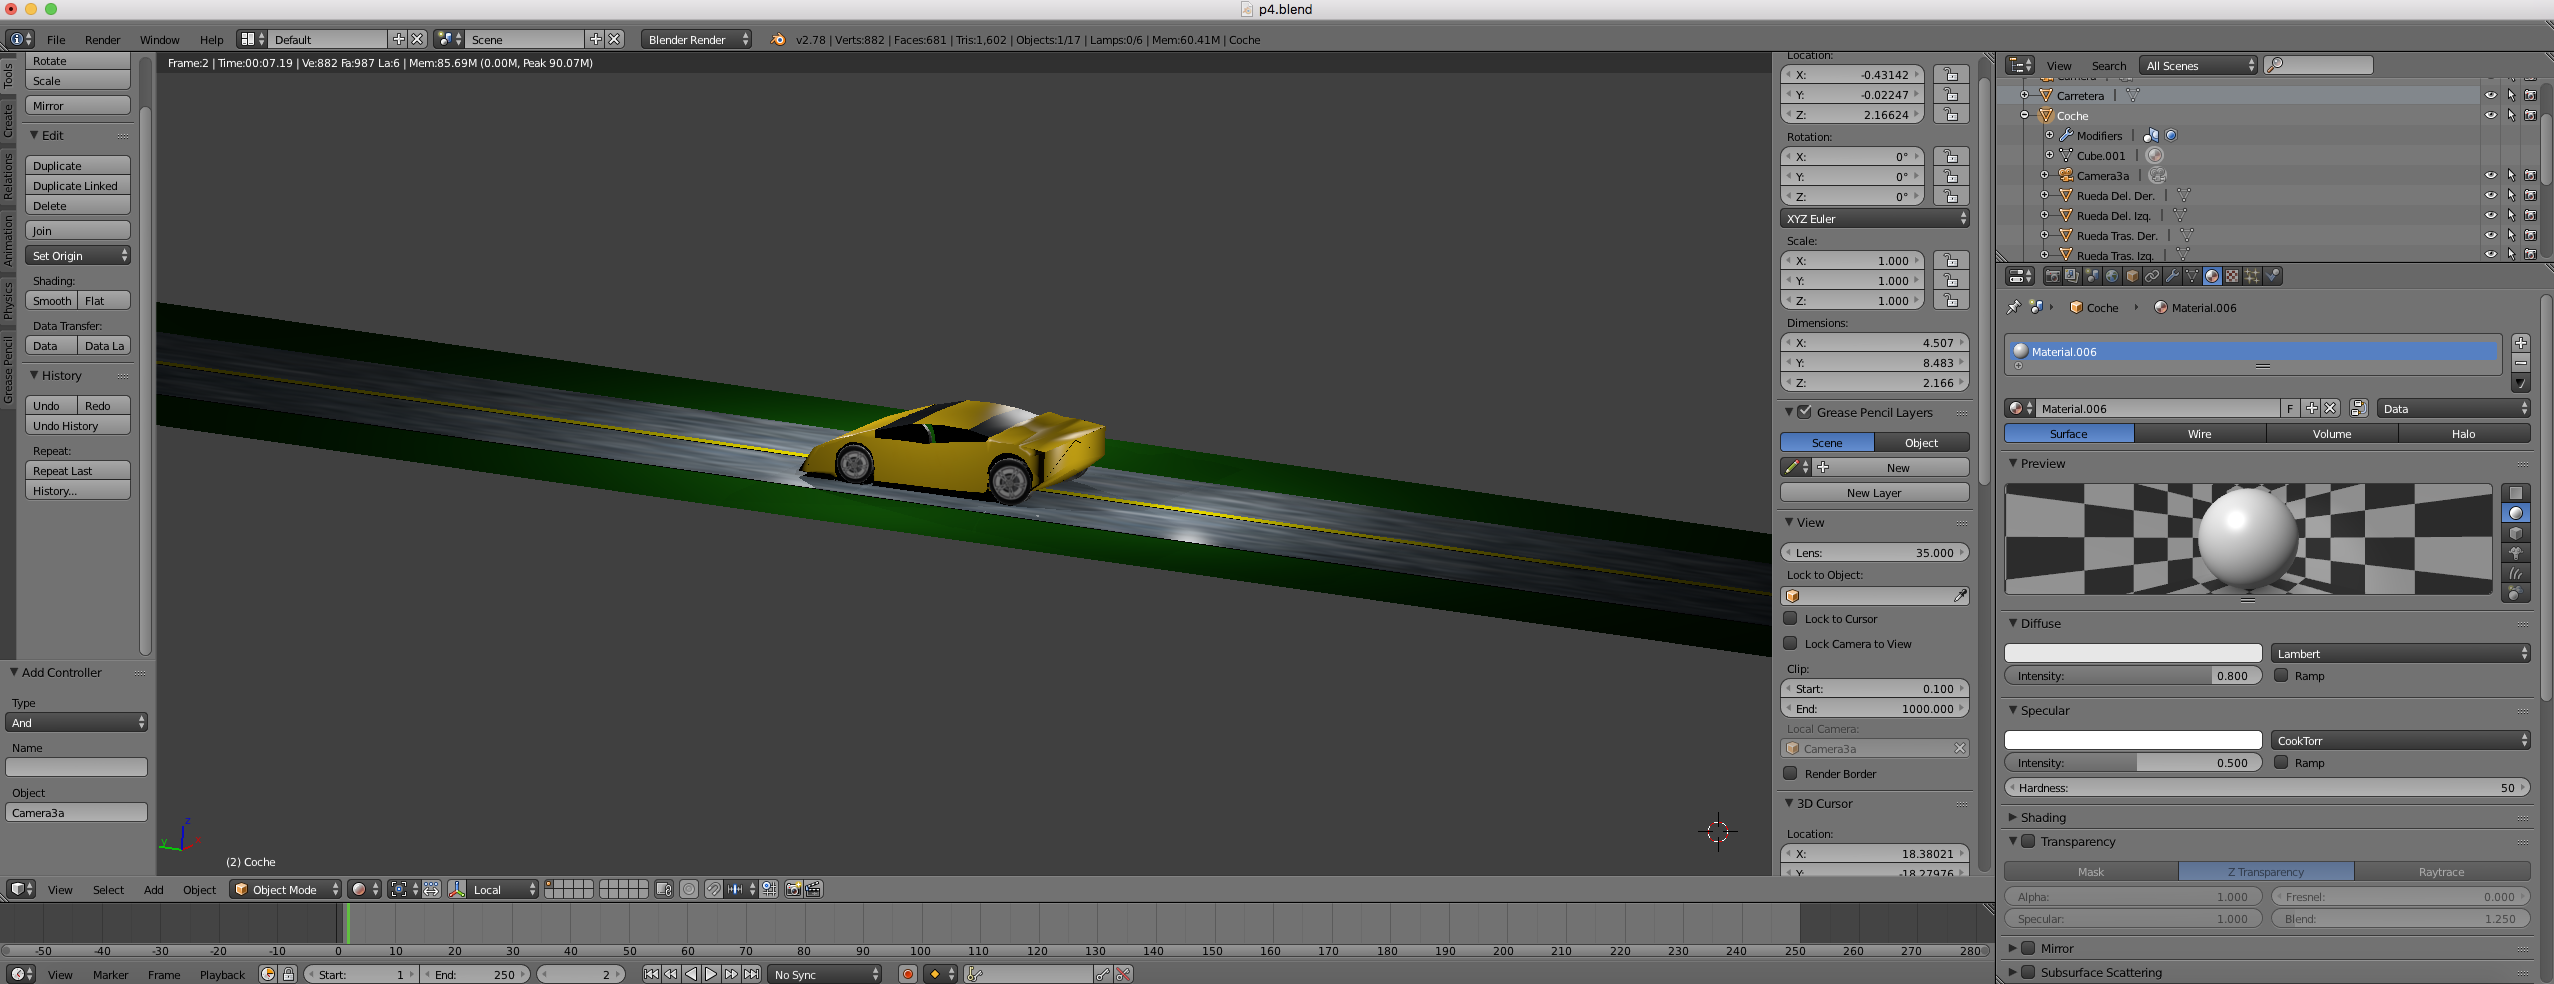
\includegraphics[width = 1.00\textwidth]{p4-img1}
 		\captionof{figure}{\label{fig:IPN}Conexion remota a \textbf{hadoop.ugr.es}.} 
	\end{center} 
\end{figure}

 \begin{figure}[H]
	\begin{center}
 		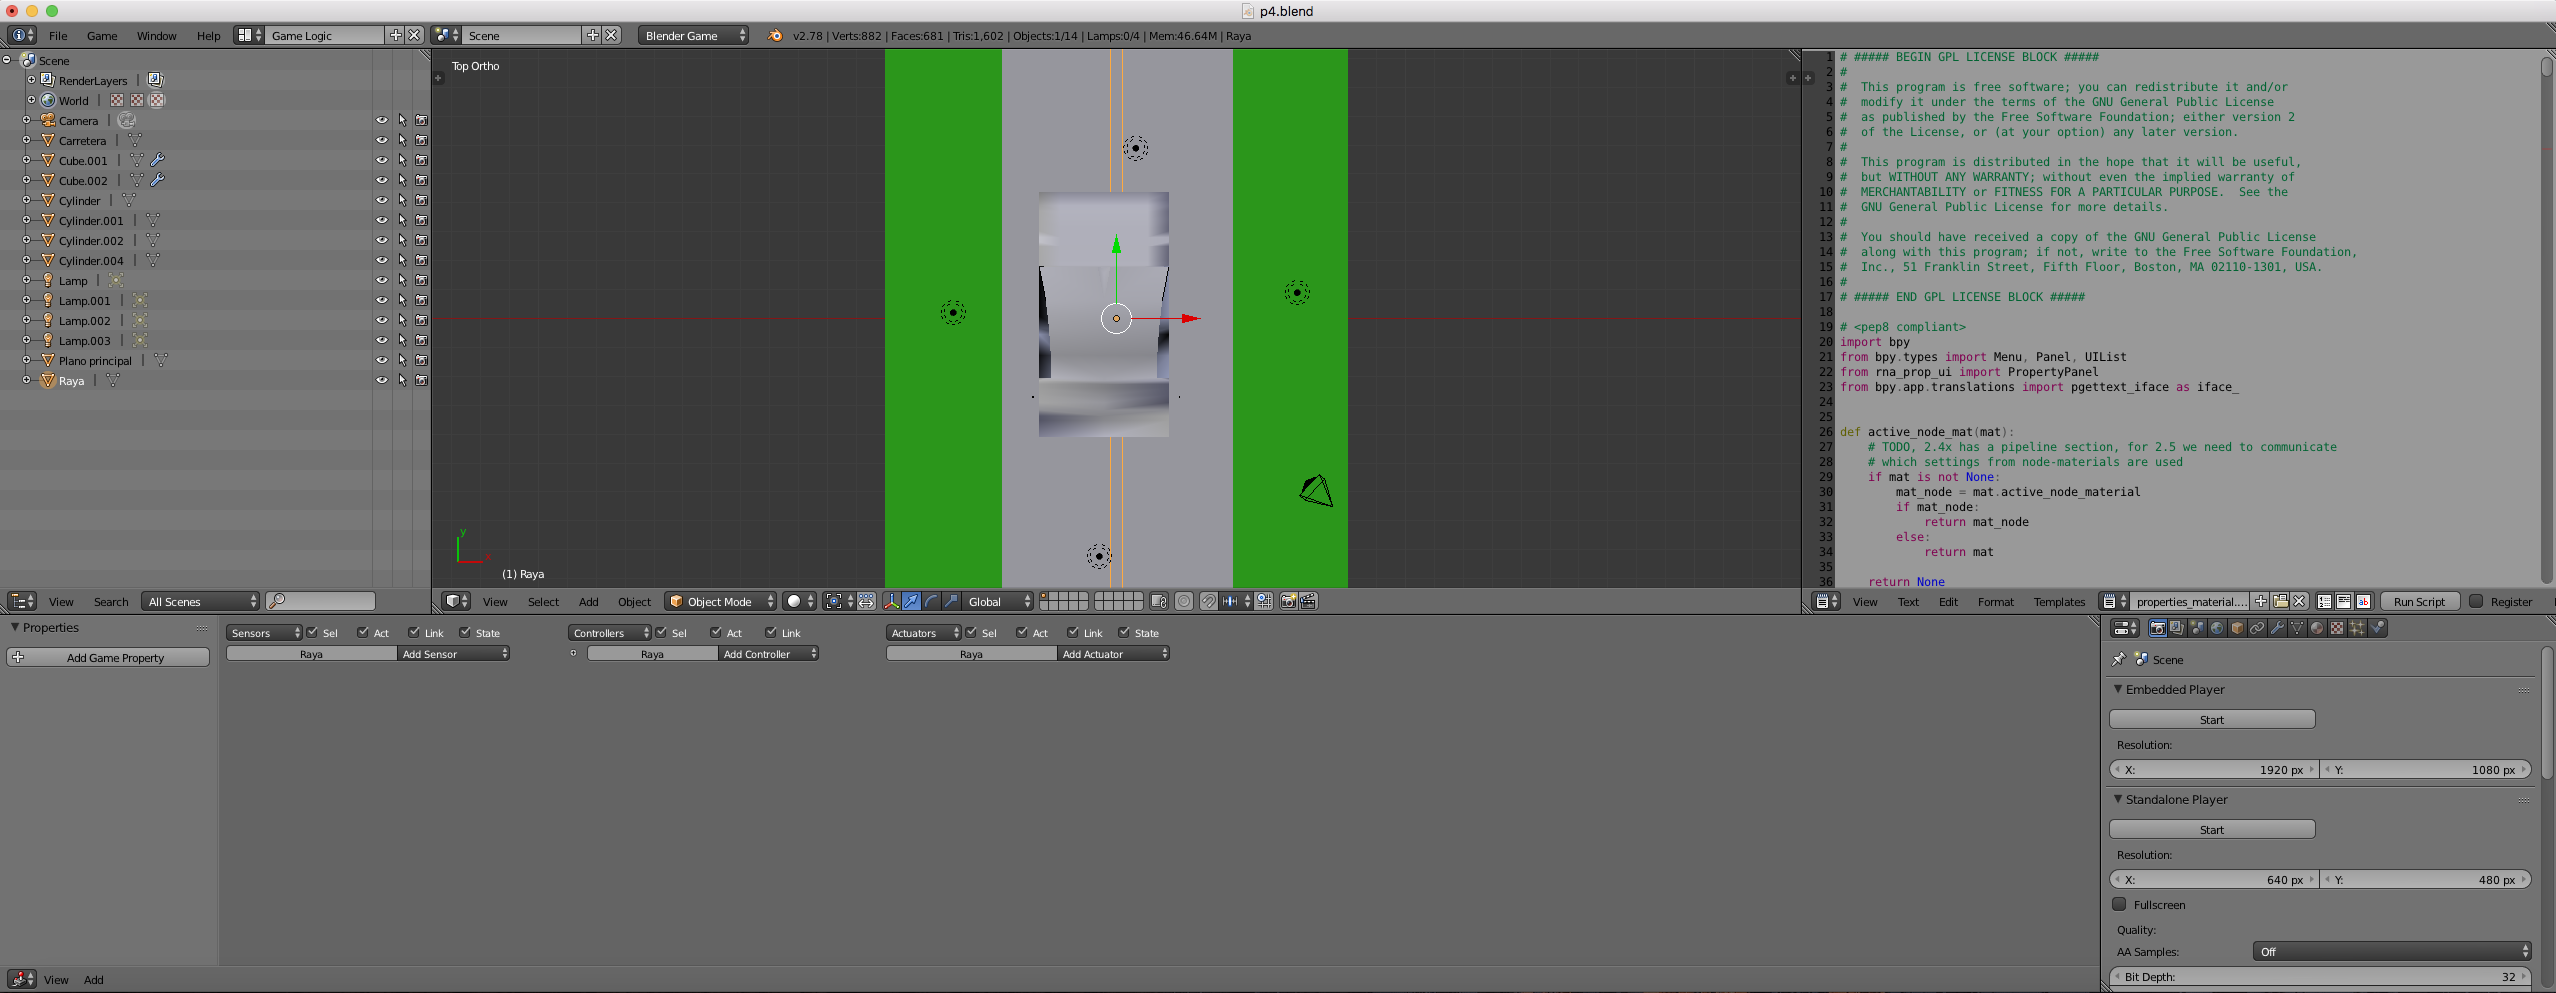
\includegraphics[width = 1.00\textwidth]{p4-img2}
 		\captionof{figure}{\label{fig:IPN}Copiando los ficheros Java.} 
	\end{center} 
\end{figure}

 \begin{figure}[H]
	\begin{center}
 		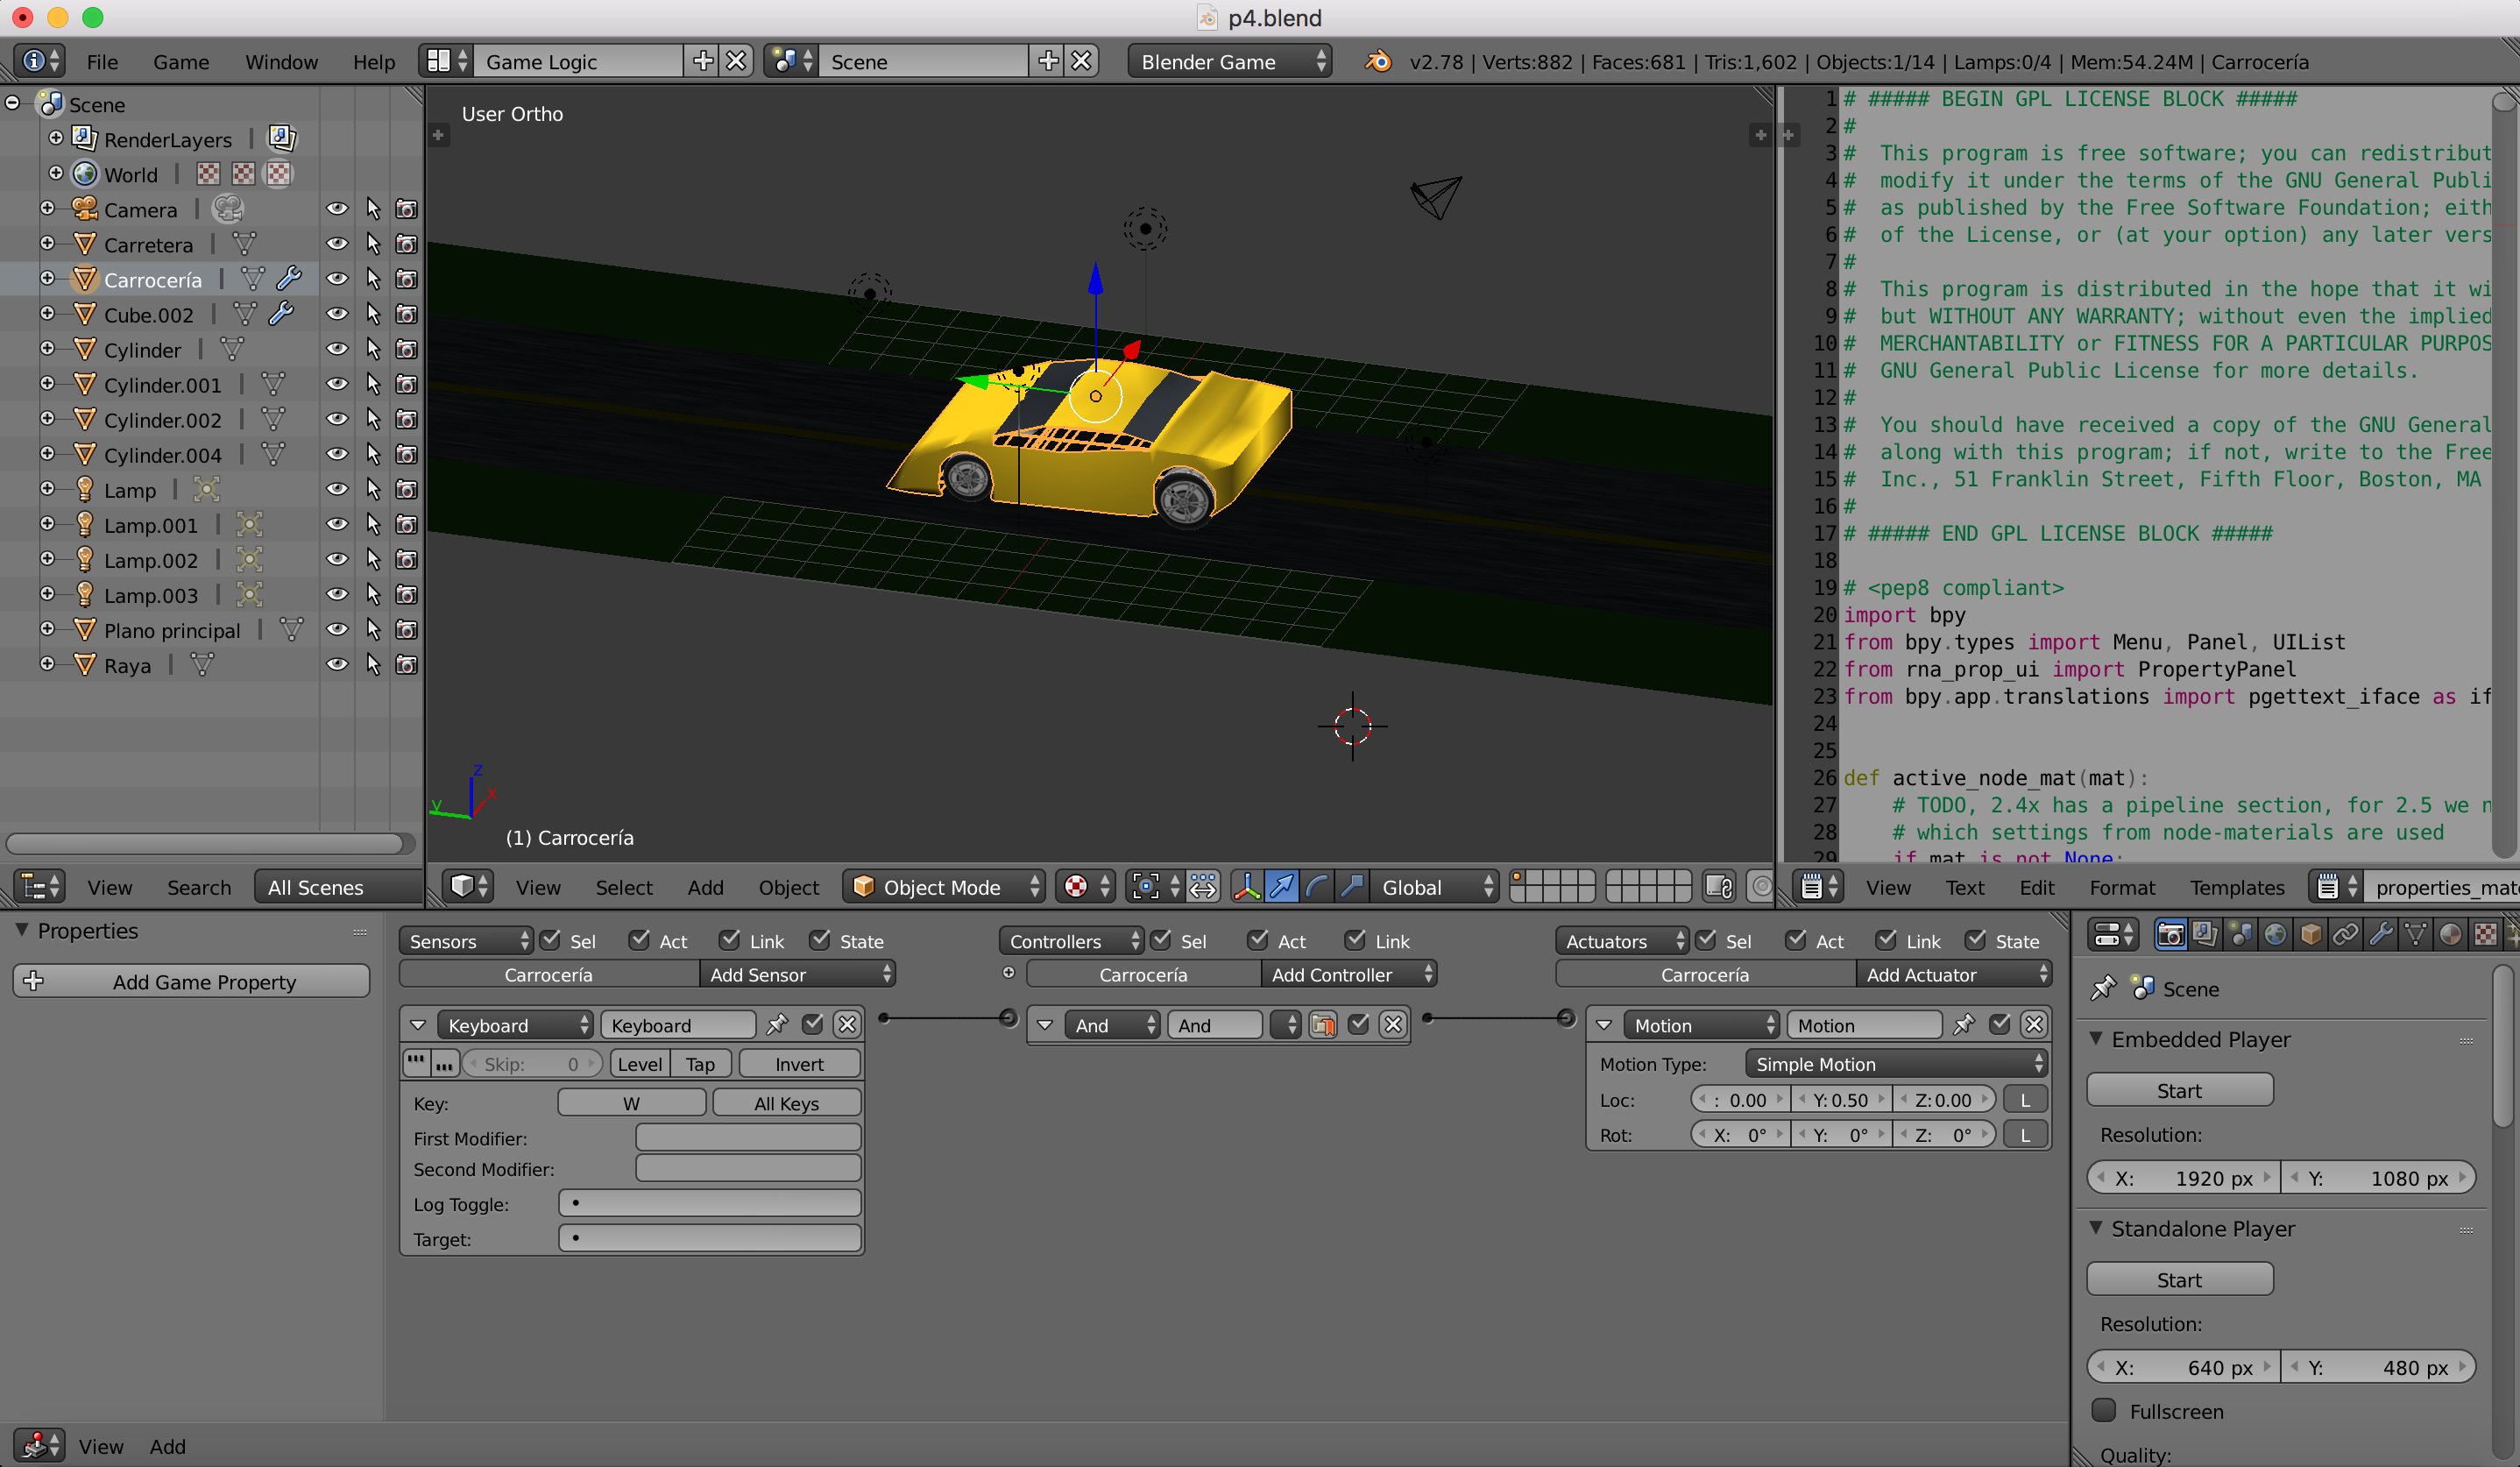
\includegraphics[width = 1.00\textwidth]{p4-img3}
 		\captionof{figure}{\label{fig:IPN}Datos de entrada.} 
	\end{center} 
\end{figure}

Viendo que están disponibles, ahora nos creamos un directorio local para las clases de java. \\

 \begin{figure}[H]
	\begin{center}
 		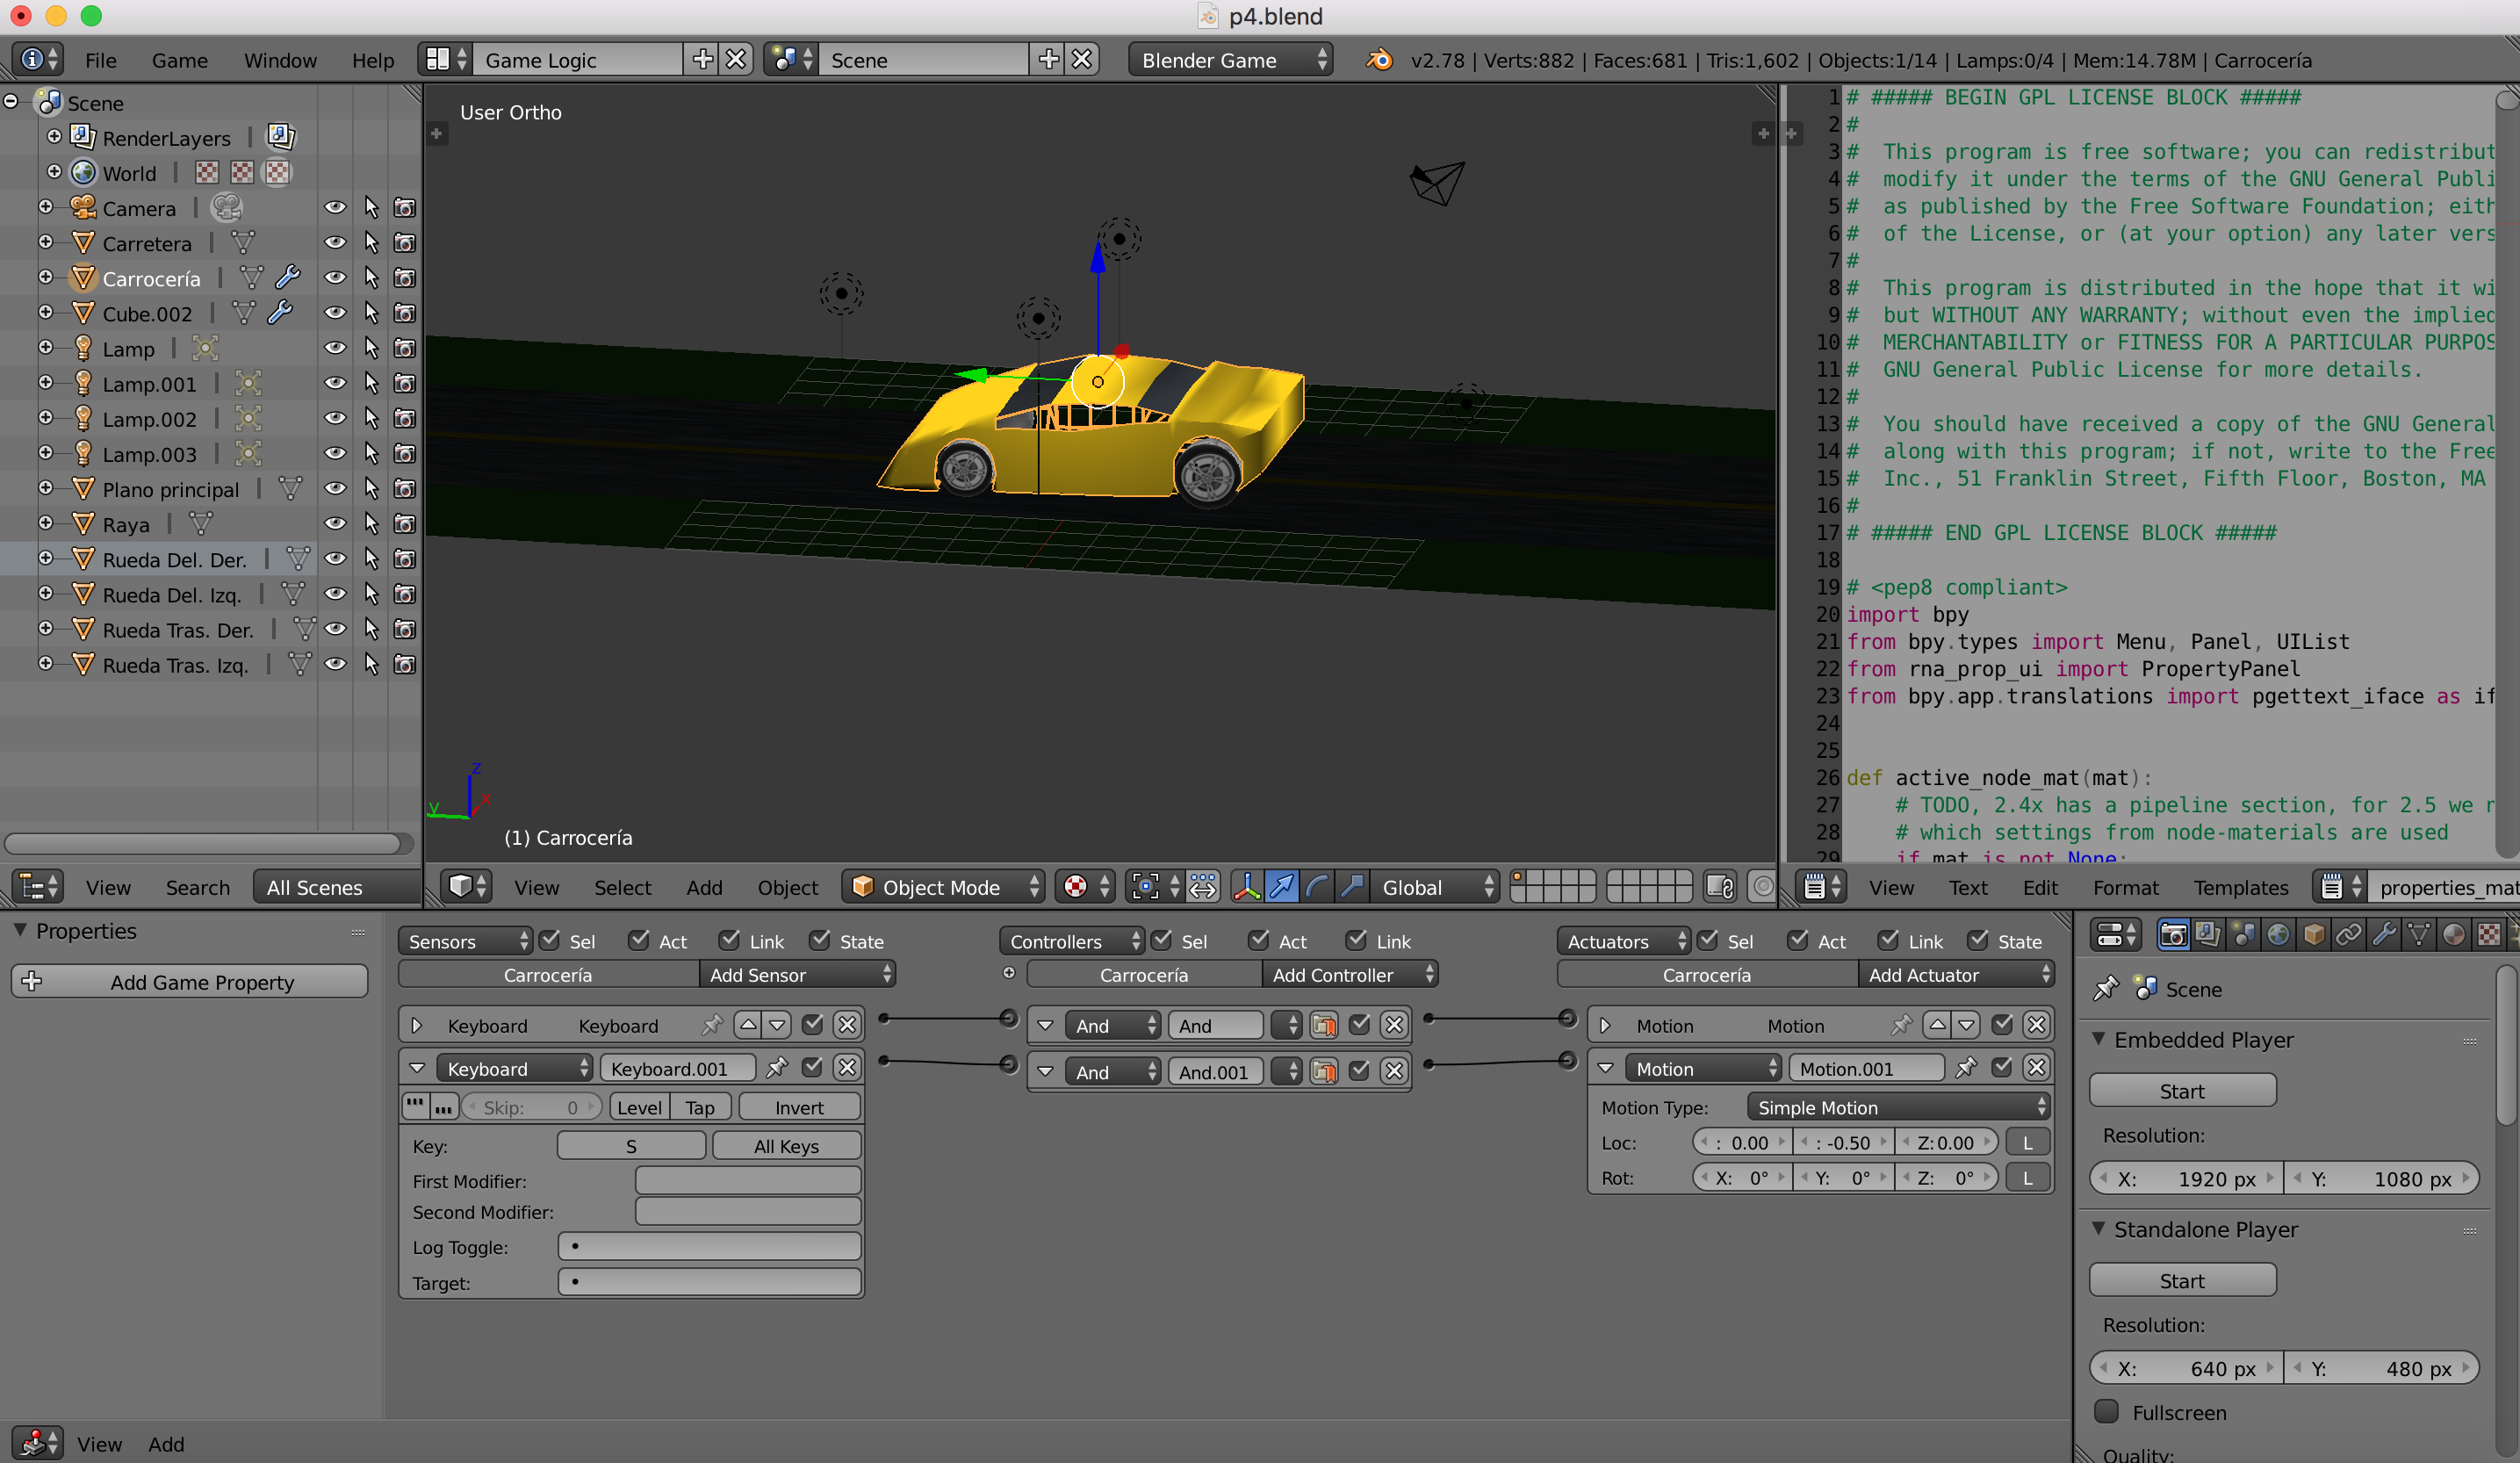
\includegraphics[width = 1.00\textwidth]{p4-img4}
 		\captionof{figure}{\label{fig:IPN}Directorio local.} 
	\end{center} 
\end{figure}

Con la preconfiguración realizada pasamos a realizar las diferentes tareas que es exponen en la práctica. \\


\section{Calcula el valor mínimo de la variable (columna) 5.} 

La primera de ellas es calcular el mínimo sobre el conjunto de valores del dataset, por lo que una vez que tenemos los ficheros java ahora toca compilarlos para crear el fichero \textbf{.jar} a continuación y ejecutarlo en \textbf{hadoop}.\\

\begin{figure}[H]
	\begin{center}
 		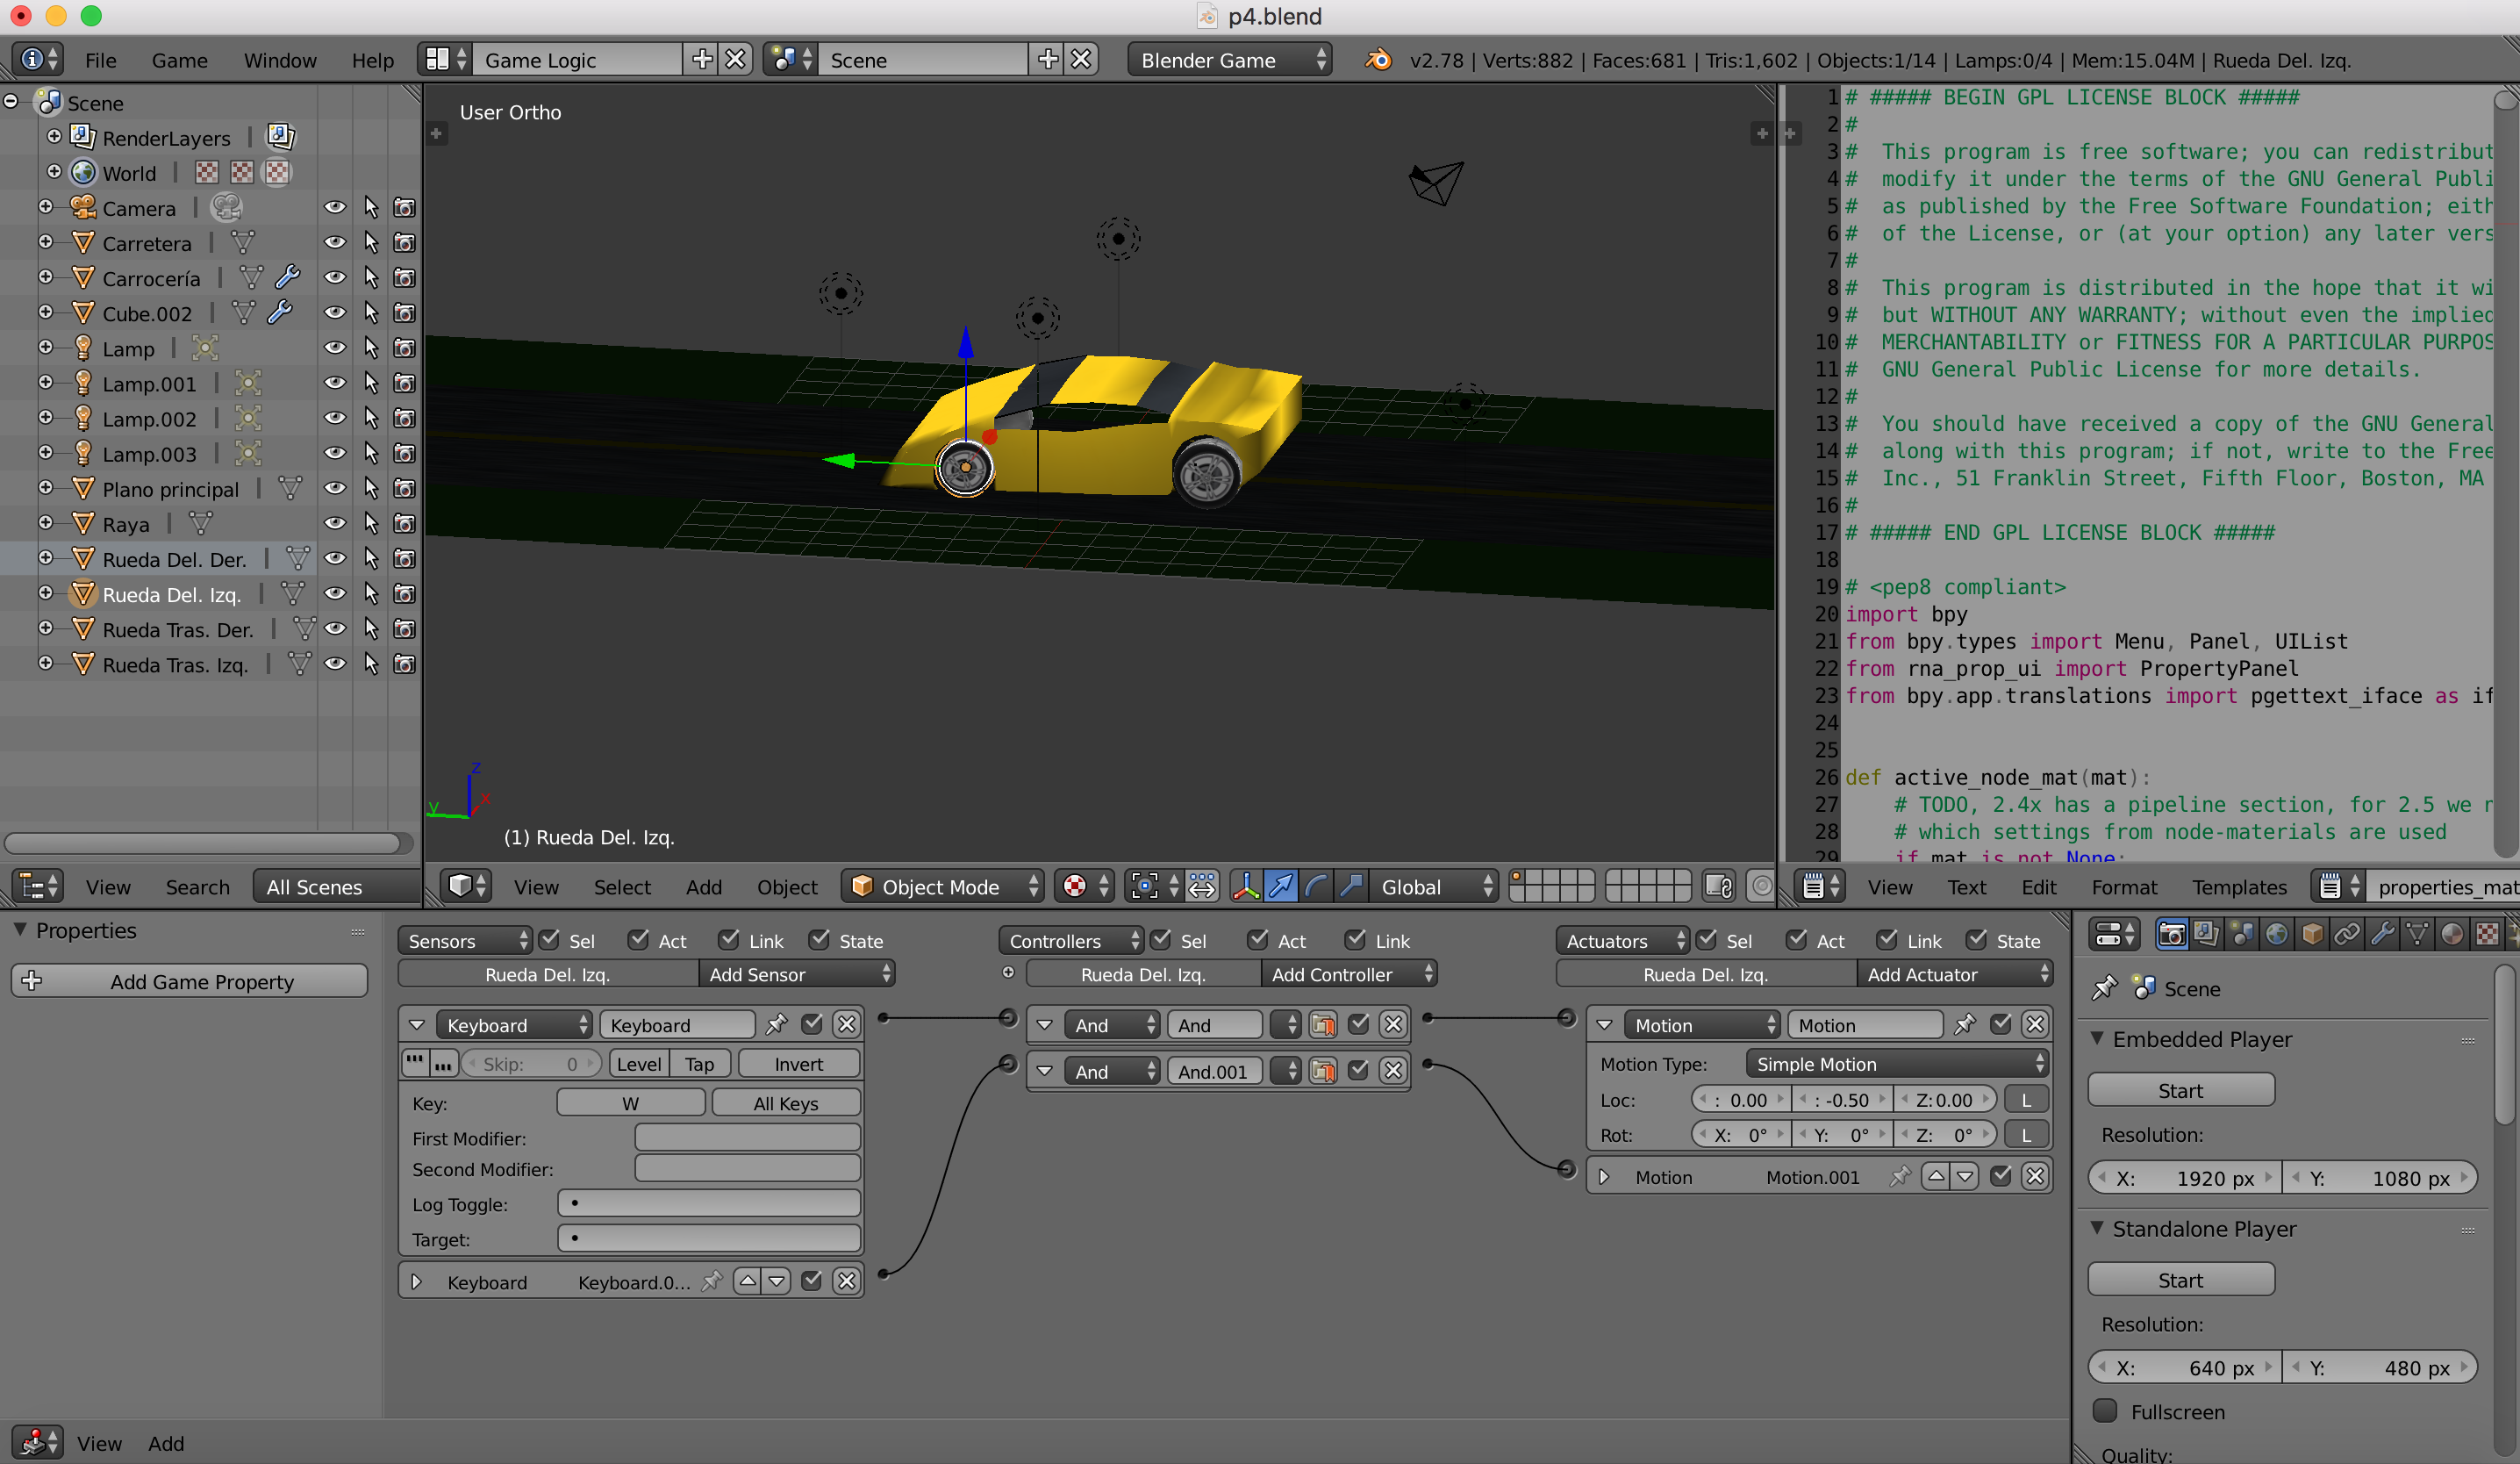
\includegraphics[width = 1.00\textwidth]{p4-img5}
 		\captionof{figure}{\label{fig:IPN}Compilamos y ejecutamos (I).} 
	\end{center} 
\end{figure}

\begin{figure}[H]
	\begin{center}
 		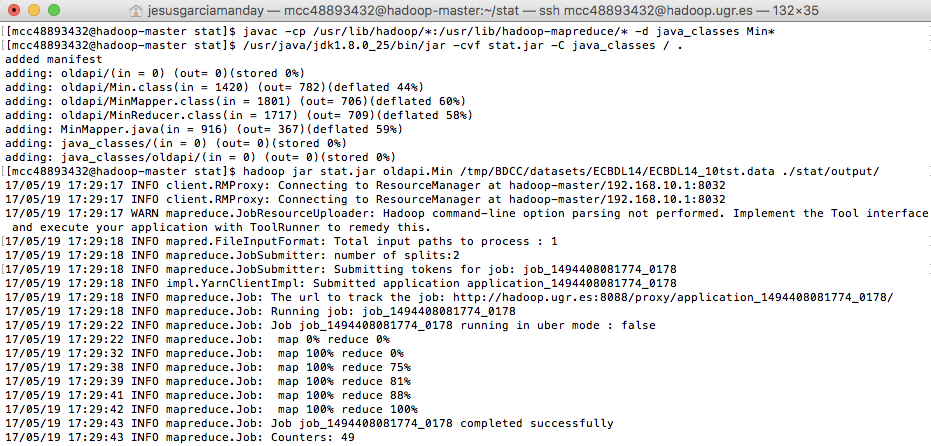
\includegraphics[width = 1.00\textwidth]{p4-img6}
 		\captionof{figure}{\label{fig:IPN}Compilamos y ejecutamos (II).} 
	\end{center} 
\end{figure}

\begin{figure}[H]
	\begin{center}
 		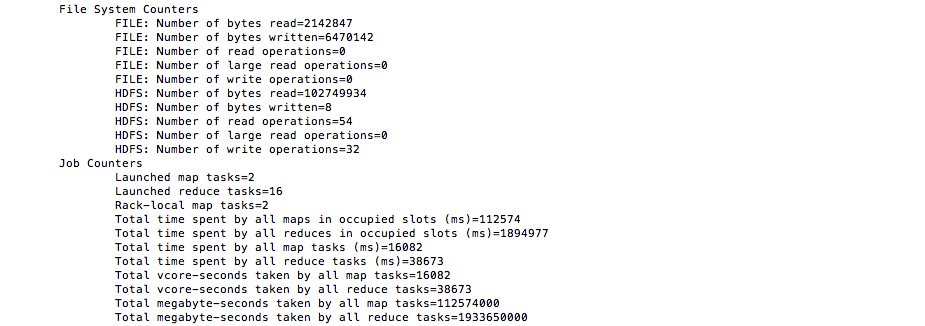
\includegraphics[width = 1.00\textwidth]{p4-img7}
 		\captionof{figure}{\label{fig:IPN}Compilamos y ejecutamos (III).} 
	\end{center} 
\end{figure}

\begin{figure}[H]
	\begin{center}
 		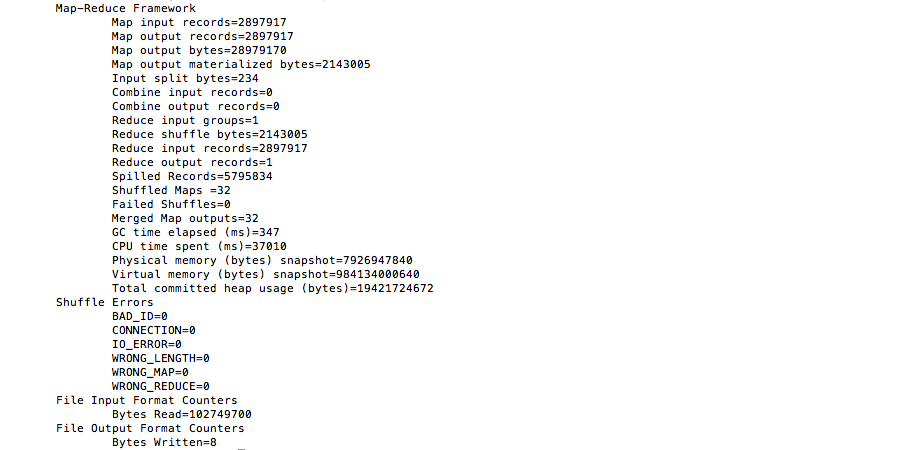
\includegraphics[width = 1.00\textwidth]{p4-img8}
 		\captionof{figure}{\label{fig:IPN}Compilamos y ejecutamos (IV).} 
	\end{center} 
\end{figure}

Por último comprobamos el resultado para ver si se ha realizado correctamente. \\

\begin{figure}[H]
	\begin{center}
 		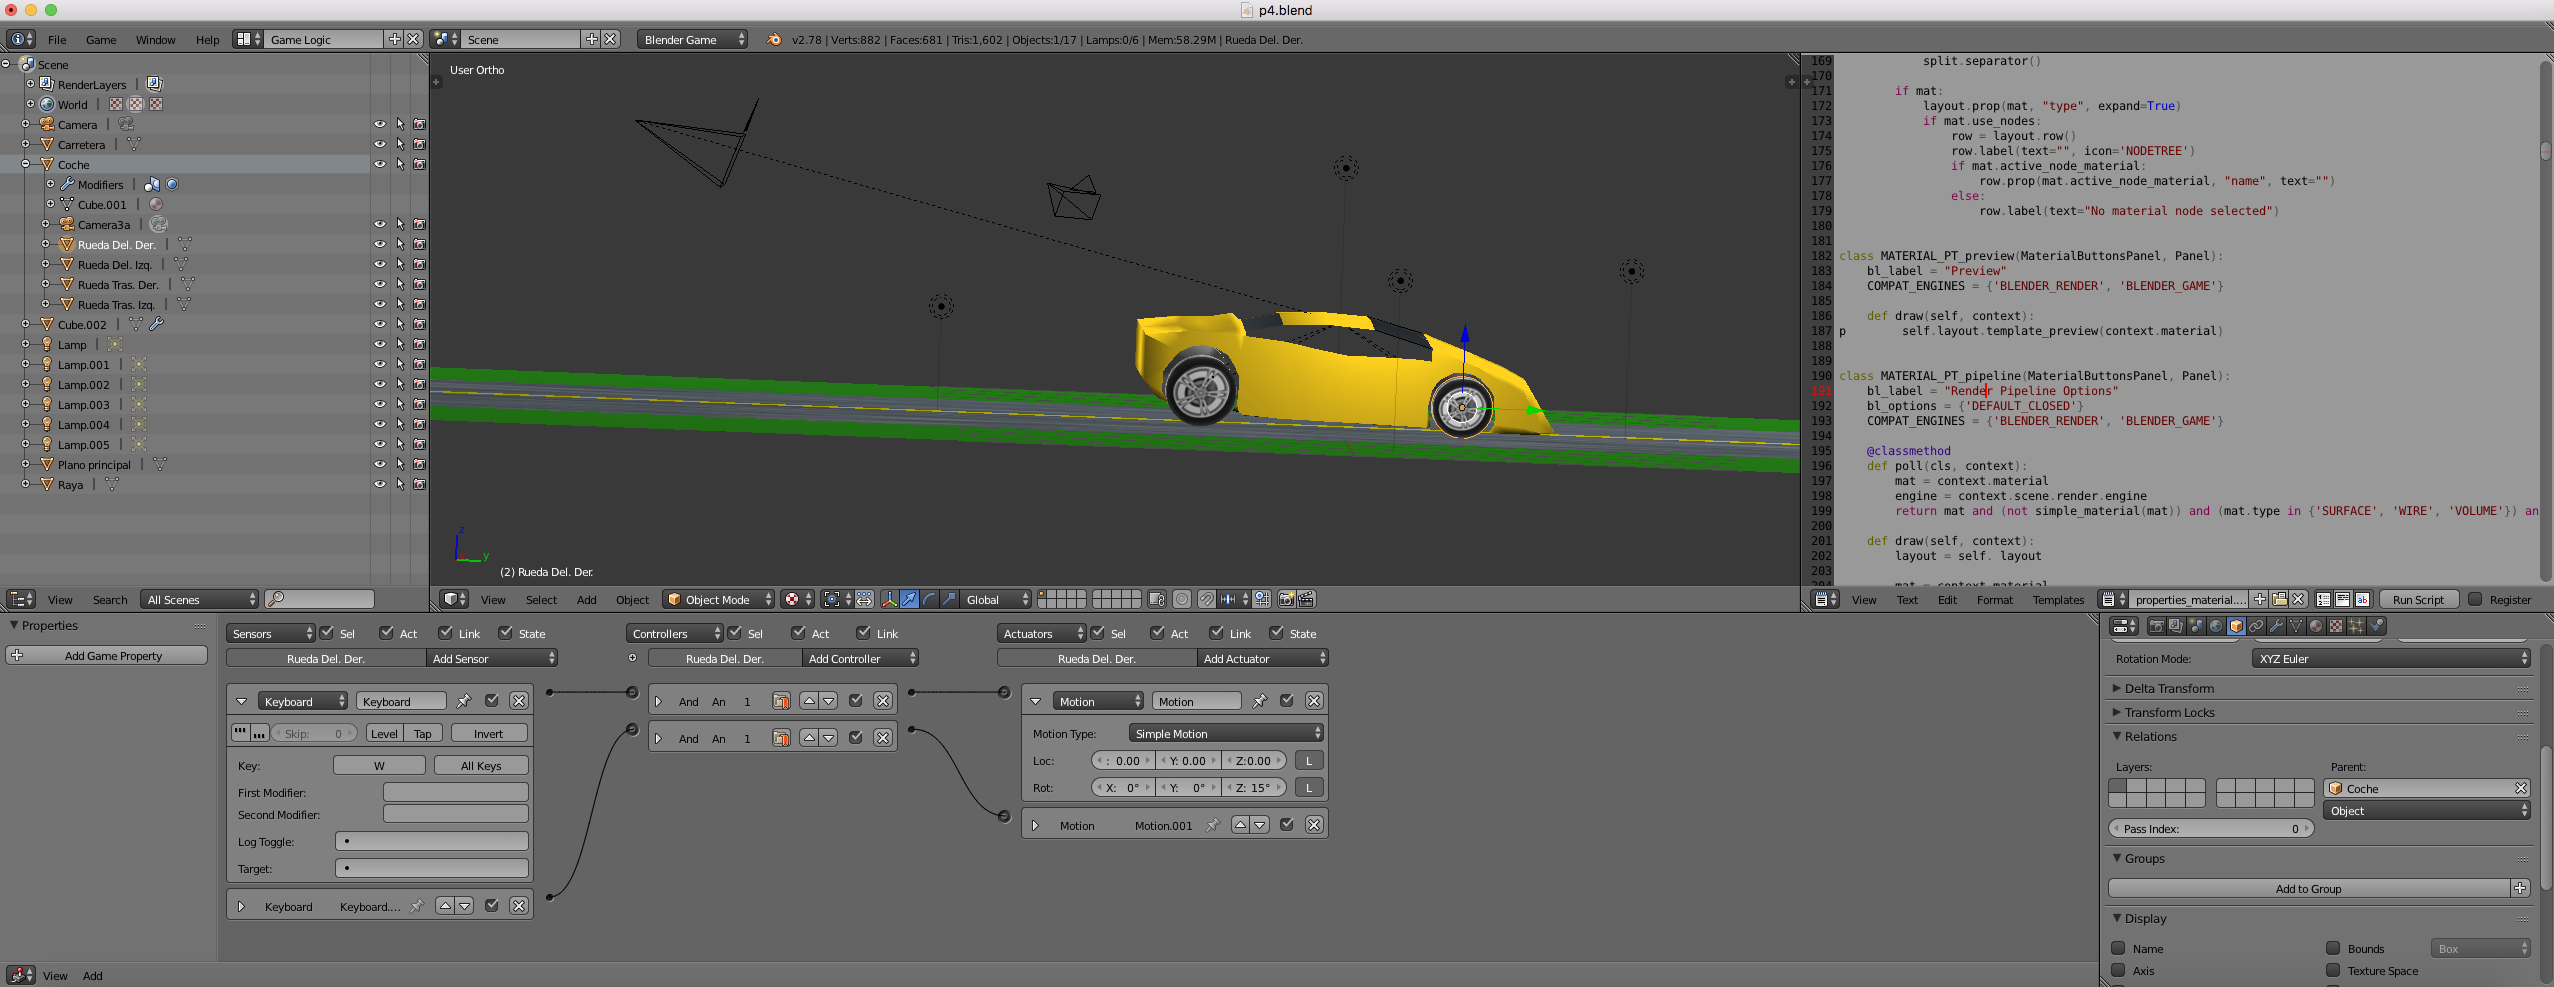
\includegraphics[width = 1.00\textwidth]{p4-img9}
 		\captionof{figure}{\label{fig:IPN}Comprobando resultado.} 
	\end{center} 
\end{figure}

\section{Calcula el valor máximo de la variable (columna) 5.} 

\section{Calcula al mismo tiempo los valores máximo y mínimo de la variable 5.} 

\section{Calcula los valores máximo y mínimo de todas las variables (salvo la última, que es la  etiqueta de la clase).} 

\section{Realizar la media de la variable 5.} 

\section{Obtener la media de todas las variables (salvo la clase).} 

\section{Comprobar si el conjunto de datos ECBDL es balanceado o no balanceado, es decir, que el ratio entre clases sea menor o mayor que 1.5 respectivamente.} 

\section{Cálculo del coeficiente de correlación entre todas las parejas de variables.} 



\end{document}